% Options for packages loaded elsewhere
\PassOptionsToPackage{unicode}{hyperref}
\PassOptionsToPackage{hyphens}{url}
\PassOptionsToPackage{dvipsnames,svgnames,x11names}{xcolor}
\documentclass[
]{article}
\usepackage{xcolor}
\usepackage[margin=1in]{geometry}
\usepackage{amsmath,amssymb}
\setcounter{secnumdepth}{-\maxdimen} % remove section numbering
\usepackage{iftex}
\ifPDFTeX
  \usepackage[T1]{fontenc}
  \usepackage[utf8]{inputenc}
  \usepackage{textcomp} % provide euro and other symbols
\else % if luatex or xetex
  \usepackage{unicode-math} % this also loads fontspec
  \defaultfontfeatures{Scale=MatchLowercase}
  \defaultfontfeatures[\rmfamily]{Ligatures=TeX,Scale=1}
\fi
\usepackage{lmodern}
\ifPDFTeX\else
  % xetex/luatex font selection
\fi
% Use upquote if available, for straight quotes in verbatim environments
\IfFileExists{upquote.sty}{\usepackage{upquote}}{}
\IfFileExists{microtype.sty}{% use microtype if available
  \usepackage[]{microtype}
  \UseMicrotypeSet[protrusion]{basicmath} % disable protrusion for tt fonts
}{}
\makeatletter
\@ifundefined{KOMAClassName}{% if non-KOMA class
  \IfFileExists{parskip.sty}{%
    \usepackage{parskip}
  }{% else
    \setlength{\parindent}{0pt}
    \setlength{\parskip}{6pt plus 2pt minus 1pt}}
}{% if KOMA class
  \KOMAoptions{parskip=half}}
\makeatother
\usepackage{longtable,booktabs,array}
\usepackage{calc} % for calculating minipage widths
% Correct order of tables after \paragraph or \subparagraph
\usepackage{etoolbox}
\makeatletter
\patchcmd\longtable{\par}{\if@noskipsec\mbox{}\fi\par}{}{}
\makeatother
% Allow footnotes in longtable head/foot
\IfFileExists{footnotehyper.sty}{\usepackage{footnotehyper}}{\usepackage{footnote}}
\makesavenoteenv{longtable}
\usepackage{graphicx}
\makeatletter
\newsavebox\pandoc@box
\newcommand*\pandocbounded[1]{% scales image to fit in text height/width
  \sbox\pandoc@box{#1}%
  \Gscale@div\@tempa{\textheight}{\dimexpr\ht\pandoc@box+\dp\pandoc@box\relax}%
  \Gscale@div\@tempb{\linewidth}{\wd\pandoc@box}%
  \ifdim\@tempb\p@<\@tempa\p@\let\@tempa\@tempb\fi% select the smaller of both
  \ifdim\@tempa\p@<\p@\scalebox{\@tempa}{\usebox\pandoc@box}%
  \else\usebox{\pandoc@box}%
  \fi%
}
% Set default figure placement to htbp
\def\fps@figure{htbp}
\makeatother
\setlength{\emergencystretch}{3em} % prevent overfull lines
\providecommand{\tightlist}{%
  \setlength{\itemsep}{0pt}\setlength{\parskip}{0pt}}
\usepackage{bookmark}
\IfFileExists{xurl.sty}{\usepackage{xurl}}{} % add URL line breaks if available
\urlstyle{same}
\hypersetup{
  pdftitle={NeuroBeat: A Validation-Locked, Energy-Accounted Spiking Network for Inter-Patient Ventricular Ectopic Beat Detection},
  pdfauthor={Valerio Merlini (independent researcher)},
  colorlinks=true,
  linkcolor={Maroon},
  filecolor={Maroon},
  citecolor={Blue},
  urlcolor={Blue},
  pdfcreator={LaTeX via pandoc}}

\title{NeuroBeat: A Validation-Locked, Energy-Accounted Spiking Network
for Inter-Patient Ventricular Ectopic Beat Detection}
\author{Valerio Merlini (independent researcher)}
\date{July 2026}

\begin{document}
\maketitle

\emph{Contact:} github.com/Talch87/neuro-beat ~·~ \emph{Code, weights,
live dashboard:} talch87.github.io/neuro-beat

\emph{Status: preprint draft. All quantitative results are from locked
runs (operating points fit only on a DS1 validation holdout; DS2 and
external databases frozen). Reference author lists verified against
source pages, except the Neurocomputing entry (secondary search, to
confirm).}

\begin{center}\rule{0.5\linewidth}{0.5pt}\end{center}

\subsection{Abstract}\label{abstract}

\textbf{Problem.} Spiking neural networks (SNNs) are of interest for
always-on cardiac monitoring because event-driven computation maps onto
low-power neuromorphic hardware. However, a large fraction of the
SNN-ECG literature reports accuracy under evaluation protocols that
inflate it, chiefly intra-patient data splits and decision thresholds
selected on the test set, and rarely reports the per-inference compute
that motivates the spiking approach.

\textbf{Approach.} We present NeuroBeat, a deliberately simple
leaky-integrate-and-fire (LIF) network for ventricular ectopic beat
(VEB) detection, and evaluate it under a conservative protocol: a
patient-disjoint inter-patient split (MIT-BIH DS1 to DS2), an operating
point fit only on a DS1 validation holdout and then frozen for all test
data, an explicit per-beat synaptic-operation (SynOps) budget, and
frozen cross-database testing on two external databases.

\textbf{Result.} A single operating point trades sensitivity against
precision (VEB sensitivity 0.894 at positive predictive value (PPV)
0.490, or 0.857 at 0.679, not both), which we attribute to calibration
variance under a small validation holdout rather than to model capacity.
A two-stage gated-ensemble cascade, in which a sparse high-recall
screener (5,987 SynOps/beat) gates a three-seed ensemble confirmer that
runs only on the roughly 27\% of beats it flags, reaches VEB sensitivity
0.923 at PPV 0.616 on DS2 within 23,385 SynOps/beat, and holds VEB
sensitivity at or above 0.90 across DS2, SVDB, and INCART under one
frozen operating point. On DS2 a patient-level bootstrap over the 22
records gives wide intervals (sensitivity 0.850 to 0.976, PPV 0.355 to
0.814), which we report as the honest uncertainty for a 22-patient test
set.

\textbf{Limitations and relevance.} SynOps is a compute proxy, not
measured hardware energy. Supraventricular (SVEB) detection on a single
lead is not achievable at usable precision in this setup and we report
it as a negative result. The contribution is not a new architecture but
a validation-locked, energy-accounted evaluation pattern and a cascade
that improves the sensitivity/PPV/energy tradeoff. This positions the
method as a candidate low-power VEB screening component for wearable or
Holter-style monitoring, not as a diagnostic system.

\begin{center}\rule{0.5\linewidth}{0.5pt}\end{center}

\subsection{1. Introduction}\label{introduction}

Long-term ambulatory ECG is increasingly recorded by wearable and patch
devices that must operate for days on a small battery. Ventricular
ectopic beats are clinically meaningful: their frequency and patterning
(for example couplets and non-sustained ventricular runs) are used in
risk stratification, and reliable beat labelling underpins Holter
reporting. A detector intended for continuous, on-device operation
therefore has two coupled requirements: it must be sensitive, because
missed ventricular beats are the costly error, and it must be
inexpensive per beat, because energy determines battery life and thermal
envelope.

Spiking networks are a candidate for this regime. They compute with
sparse binary events, and on neuromorphic substrates the dominant cost
is the number of synaptic operations actually triggered by spikes rather
than a fixed clocked cost per layer. This has motivated a body of
SNN-ECG work. Our reading of that literature, consistent with a recent
systematic review {[}Silva2025{]}, is that two recurring issues limit
how far its accuracy numbers can be trusted for deployment.

First, evaluation is frequently optimistic. Under an intra-patient
split, beats from the same patient appear in both training and test
sets, so the model can exploit patient-specific morphology that a device
deployed on a new patient never observes; reported accuracy then
overstates real inter-patient performance. Separately, selecting the
decision threshold (or per-class bias) on the test set leaks label
information that is unavailable at deployment time, again inflating the
headline metric. Neither practice is exotic; both are common enough that
cross-study comparison is unreliable {[}Silva2025{]}.

Second, energy is usually not accounted for. The stated reason to use an
SNN is efficiency, yet many reports give only accuracy or parameter
counts, with no per-inference operation budget against which efficiency
could be judged.

The contribution of this paper is therefore not a novel architecture.
The network is intentionally small and conventional. The contribution is
evaluation discipline and an energy-accounted deployment framing: an
operating point that is locked on validation data and never touched on
test data, an explicit SynOps budget applied to every configuration,
frozen cross-database testing, and a gated cascade that improves the
sensitivity/PPV/energy tradeoff within that budget. We also report,
rather than hide, a clear negative result for supraventricular beats on
a single lead.

\textbf{Contributions.}

\begin{enumerate}
\def\labelenumi{\arabic{enumi}.}
\tightlist
\item
  \textbf{A validation-locked inter-patient protocol.} We adopt the de
  Chazal DS1/DS2 patient-disjoint split {[}deChazal2004{]}, hold out
  three DS1 records as a patient-disjoint validation set, fit the
  operating point only on that holdout, and freeze it for DS2 and all
  external data. No reported test number participates in selecting the
  operating point on the split it is reported on (Section 6).
\item
  \textbf{An explicit per-beat SynOps budget.} We define a per-beat
  synaptic-operation count (Section 5.4), report it for every
  configuration, and hold each to a fixed 25,000 SynOps/beat budget.
\item
  \textbf{Frozen cross-database validation.} The single frozen operating
  point is applied unchanged to two databases the model never trained on
  (SVDB, INCART), quantifying transfer under distribution shift.
\item
  \textbf{A gated-ensemble cascade within budget.} A sparse screener on
  every beat gates a small ensemble confirmer on flagged beats, reaching
  VEB sensitivity 0.923 at PPV 0.616 within 23,385 SynOps/beat, which no
  single-stage model in our sweep achieves.
\item
  \textbf{A negative result for single-lead SVEB.} Under the same
  protocol, single-lead supraventricular detection does not reach usable
  precision, and we document why and how it fails rather than tuning it
  to a misleading number.
\end{enumerate}

\begin{center}\rule{0.5\linewidth}{0.5pt}\end{center}

\subsection{2. Related Work}\label{related-work}

\textbf{(a) ECG arrhythmia classification and inter-patient evaluation.}
The ANSI/AAMI EC57 standard {[}AAMI-EC57{]} defines the five heartbeat
classes and the sensitivity/PPV reporting convention used throughout
this literature. de Chazal et al.~{[}deChazal2004{]} introduced the
patient-disjoint DS1/DS2 partition of the 44 non-paced MIT-BIH records
(about 50,000 beats per set) that has become the reference inter-patient
benchmark. Many subsequent methods report higher raw accuracy than we
do, but a substantial share do so under intra-patient splits or with
test-set-selected thresholds; the systematic review of Silva et al.
{[}Silva2025{]} documents that few studies simultaneously satisfy
inter-patient partitioning, AAMI compliance, and embedded feasibility.
We do not claim to beat the strongest reported numbers on raw accuracy;
we claim comparability under a stricter, leakage-controlled protocol
with an energy budget.

\textbf{(b) Low-power and embedded ECG inference.} A parallel line of
work targets resource-constrained deployment through quantized and
compact convolutional or temporal-convolutional models, pruning, and
microcontroller implementations. These approaches report MACs, memory
footprint, or measured microcontroller energy. They are the natural
non-spiking comparison point for efficiency claims; we include
convolutional and recurrent baselines here (Section 7.5) and note
quantized CNN and temporal-convolutional baselines as needed additional
comparisons (Section 9).

\textbf{(c) Spiking and neuromorphic ECG.} SNN-ECG methods report
competitive MIT-BIH accuracy using delta-modulation encoding of the ECG
and its derivatives {[}SNN-ECG-BSPC2021{]}, spike-driven processors for
wearable ECG {[}Chu2022{]}, hardware/software co-design
{[}SparrowSNN2024{]}, and axonal-delay models {[}AxonalDelays2025{]}.
Our count-pooled delta encoding over signal orders is in this family. We
differ in evaluation rather than in mechanism: we report validation-
locked inter-patient results with an explicit SynOps budget, frozen
cross-database transfer, and a documented single-lead SVEB failure.

\textbf{(d) Cascaded and gated inference.} Two-stage screener/confirmer
and energy-gated designs are established elsewhere for trading average
compute against accuracy. We use the pattern narrowly: to make an
ensemble-grade confirmer affordable on average by invoking it only on
candidates a cheap screener flags.

\textbf{(e) Evaluation hygiene and reproducibility.} Our protocol
choices follow the recommendations surveyed in {[}Silva2025{]}. We
additionally release code, frozen weights, per-seed logs, and a public
results page so that every reported number is regenerable.

\begin{center}\rule{0.5\linewidth}{0.5pt}\end{center}

\subsection{3. Data}\label{data}

\textbf{MIT-BIH Arrhythmia Database (primary).} 48 two-lead ambulatory
records sampled at 360 Hz. Annotated beats are mapped to the five AAMI
classes: N (normal), S (supraventricular ectopic, SVEB), V (ventricular
ectopic, VEB), F (fusion of normal and ventricular), and Q
(unknown/paced). We use the de Chazal patient-disjoint split
{[}deChazal2004{]}: DS1 for training and DS2 for test, with no patient
in both. From DS1 we hold out records 201, 207, and 223 as a
patient-disjoint validation set used only for operating-point selection.
Beat counts are given in Table 1.

\textbf{External databases (test-only).} The MIT-BIH Supraventricular
Arrhythmia Database (SVDB, 128 Hz) and the St.~Petersburg INCART 12-lead
Arrhythmia Database (INCART, 257 Hz). These are used exclusively for
frozen cross-database testing; no external beat enters training or
operating-point selection for the VEB models.

\textbf{Preprocessing and resampling.} External signals are resampled to
360 Hz with polyphase resampling (\texttt{scipy.signal.resample\_poly},
applied to the ratio reduced by its greatest common divisor), and
annotation sample indices are rescaled by the same factor. Lead
selection is fixed a priori: MIT-BIH and SVDB use lead 0; INCART uses
lead II (index 1). We apply no per-record adaptive filtering or
denoising beyond resampling, so that the reported transfer reflects the
raw morphology difference across databases.

\textbf{Beat segmentation and RR features.} Each beat is a fixed window
of 256 samples (about 0.71 s at 360 Hz) centred on the annotated R-peak;
we use provided annotations and do not run a separate detector, so
results are conditional on accurate R-peak locations (Section 9). For
each beat we compute three RR-interval features (previous RR, following
RR, and their ratio). RR features are standardized using training-set
statistics only, and the same statistics are applied unchanged to
validation, test, and external data.

\textbf{Table 1. Beat counts by class (after segmentation).}

\begin{longtable}[]{@{}lrrrrrr@{}}
\toprule\noalign{}
Split & Total & N & SVEB (S) & VEB (V) & F & Q \\
\midrule\noalign{}
\endhead
\bottomrule\noalign{}
\endlastfoot
DS1 train & 44,573 & 38,113 & 673 & 3,255 & 2,526 & 6 \\
DS1 val (201/207/223) & 6,427 & 5,222 & 308 & 881 & 16 & 0 \\
DS2 test & 49,693 & 44,241 & 1,837 & 3,220 & 388 & 7 \\
SVDB (external) & 184,520 & 162,281 & 12,196 & 9,941 & 23 & 79 \\
INCART (external) & 175,811 & 153,621 & 1,959 & 20,006 & 219 & 6 \\
\end{longtable}

\emph{(DS1 train class counts are from the same segmentation pipeline;
the VEB and SVEB minorities are the quantities that matter for the
class-weighted objective.)}

\begin{center}\rule{0.5\linewidth}{0.5pt}\end{center}

\subsection{4. Figures}\label{figures}

Figures 1 to 5 are rendered from the locked results and included below
(sources in \texttt{paper/figures/}).

\begin{figure}
\centering
\pandocbounded{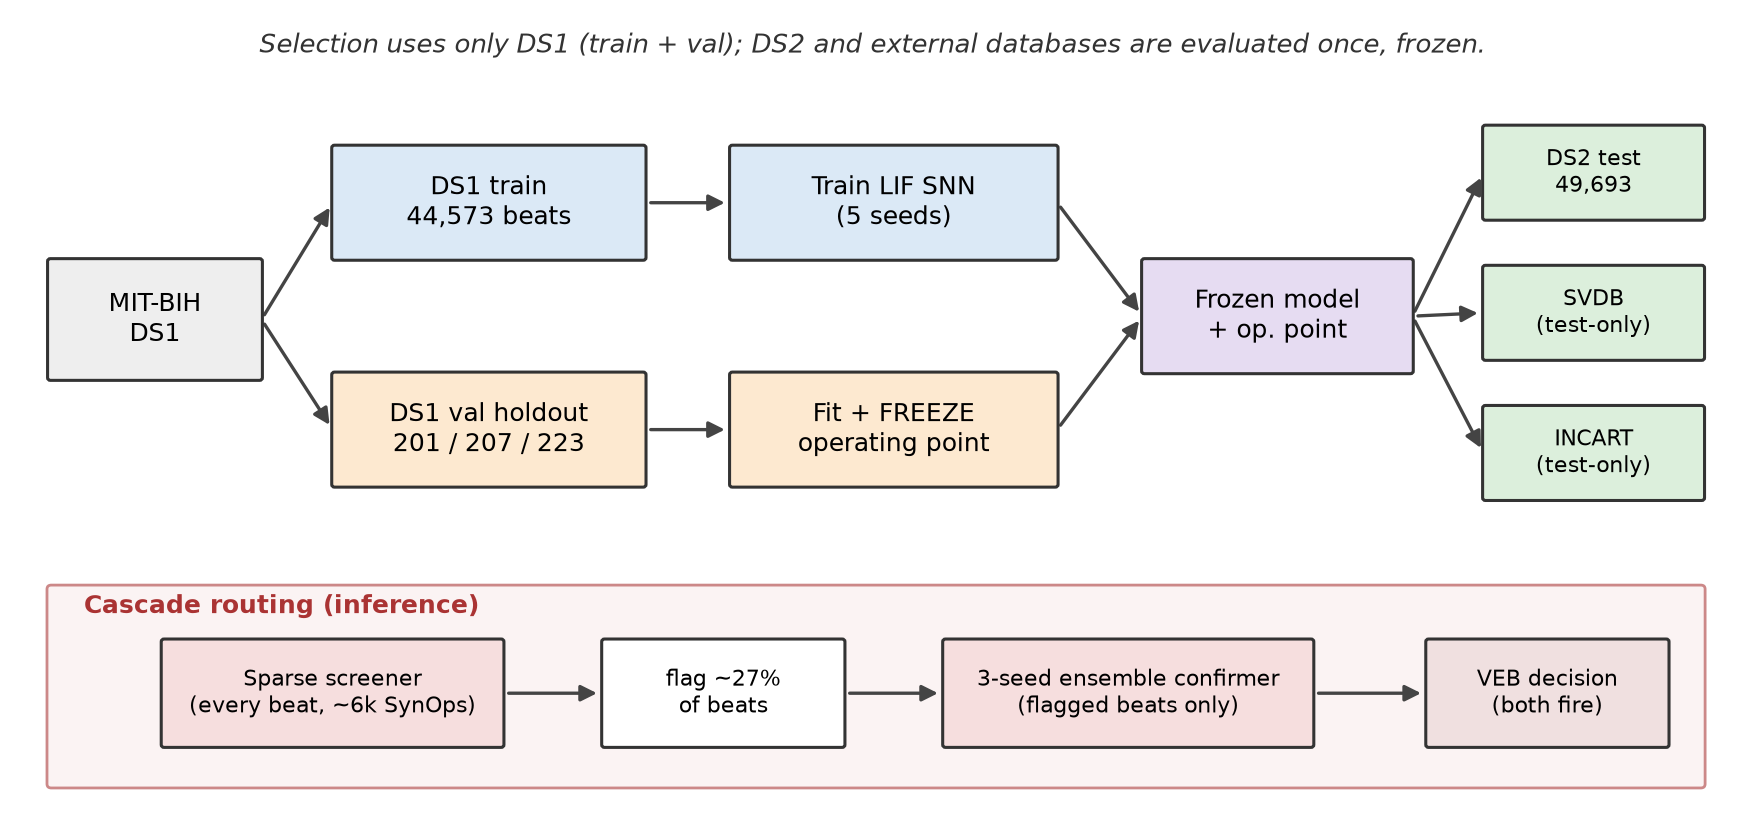
\includegraphics[keepaspectratio]{figures/fig1_protocol.png}}
\caption{Figure 1}
\end{figure}

\textbf{Figure 1 (protocol / no-leakage).} DS1 is split into a training
set and a patient-disjoint validation holdout (records 201, 207, 223).
The operating point is selected only on the validation holdout and then
frozen. The frozen model is applied once to DS2 and, unchanged, to the
external SVDB and INCART databases. The lower band shows cascade routing
at inference (sparse screener on every beat; ensemble confirmer only on
flagged beats). \emph{Message: no test or external data participates in
model or threshold selection.}

\begin{figure}
\centering
\pandocbounded{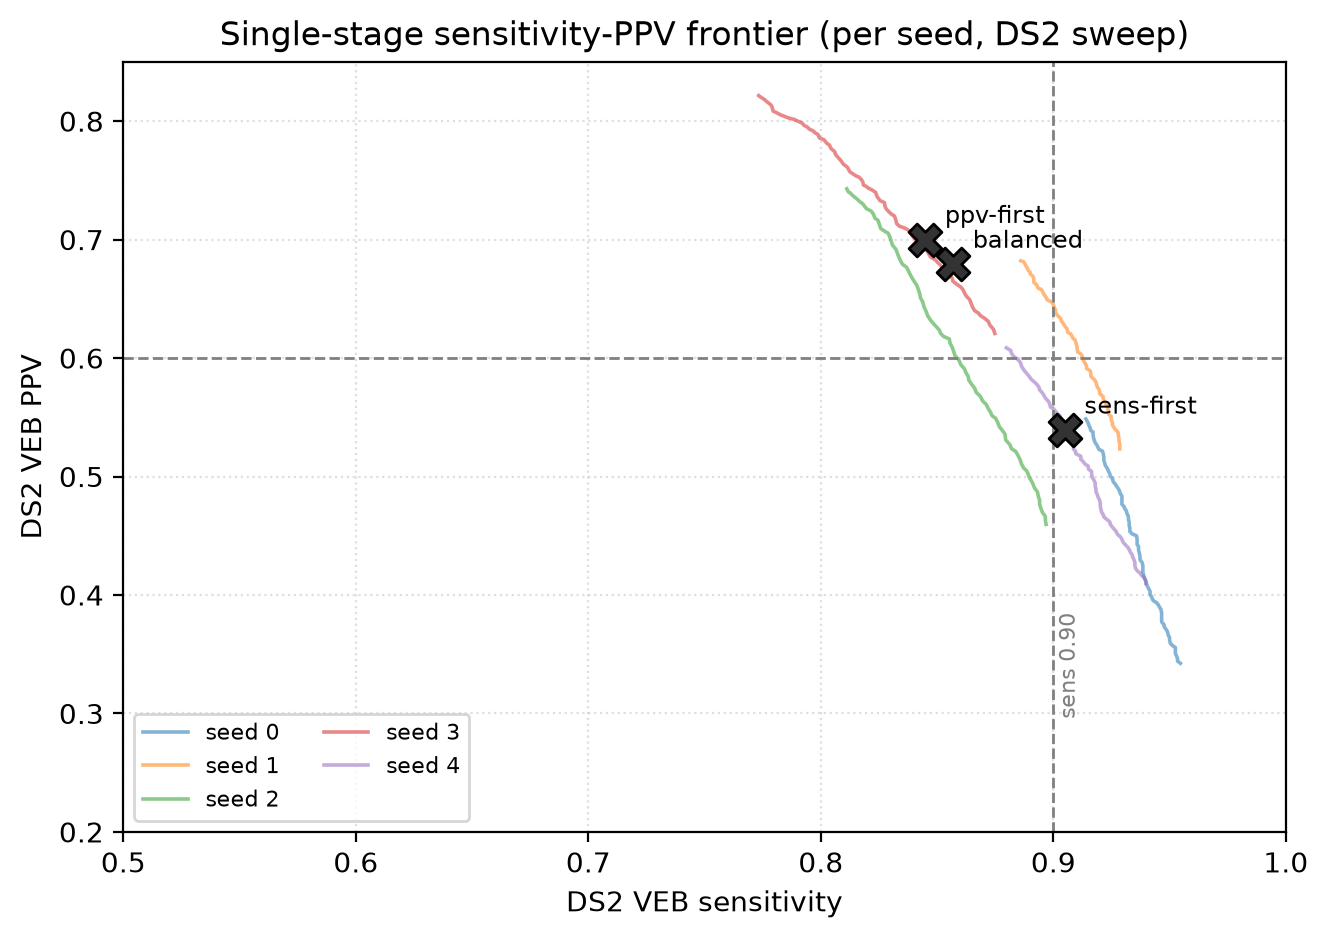
\includegraphics[keepaspectratio]{figures/fig2_frontier.png}}
\caption{Figure 2}
\end{figure}

\textbf{Figure 2 (single-stage sensitivity-PPV frontier).} DS2 VEB PPV
versus sensitivity for single-stage models, one curve per seed (DS2
threshold sweep), with the three validation-locked operating points
marked and the 0.90 and 0.60 target lines. \emph{Message: no single
operating point reaches both sensitivity \textgreater= 0.90 and PPV
\textgreater= 0.60 reliably across seeds.}

\begin{figure}
\centering
\pandocbounded{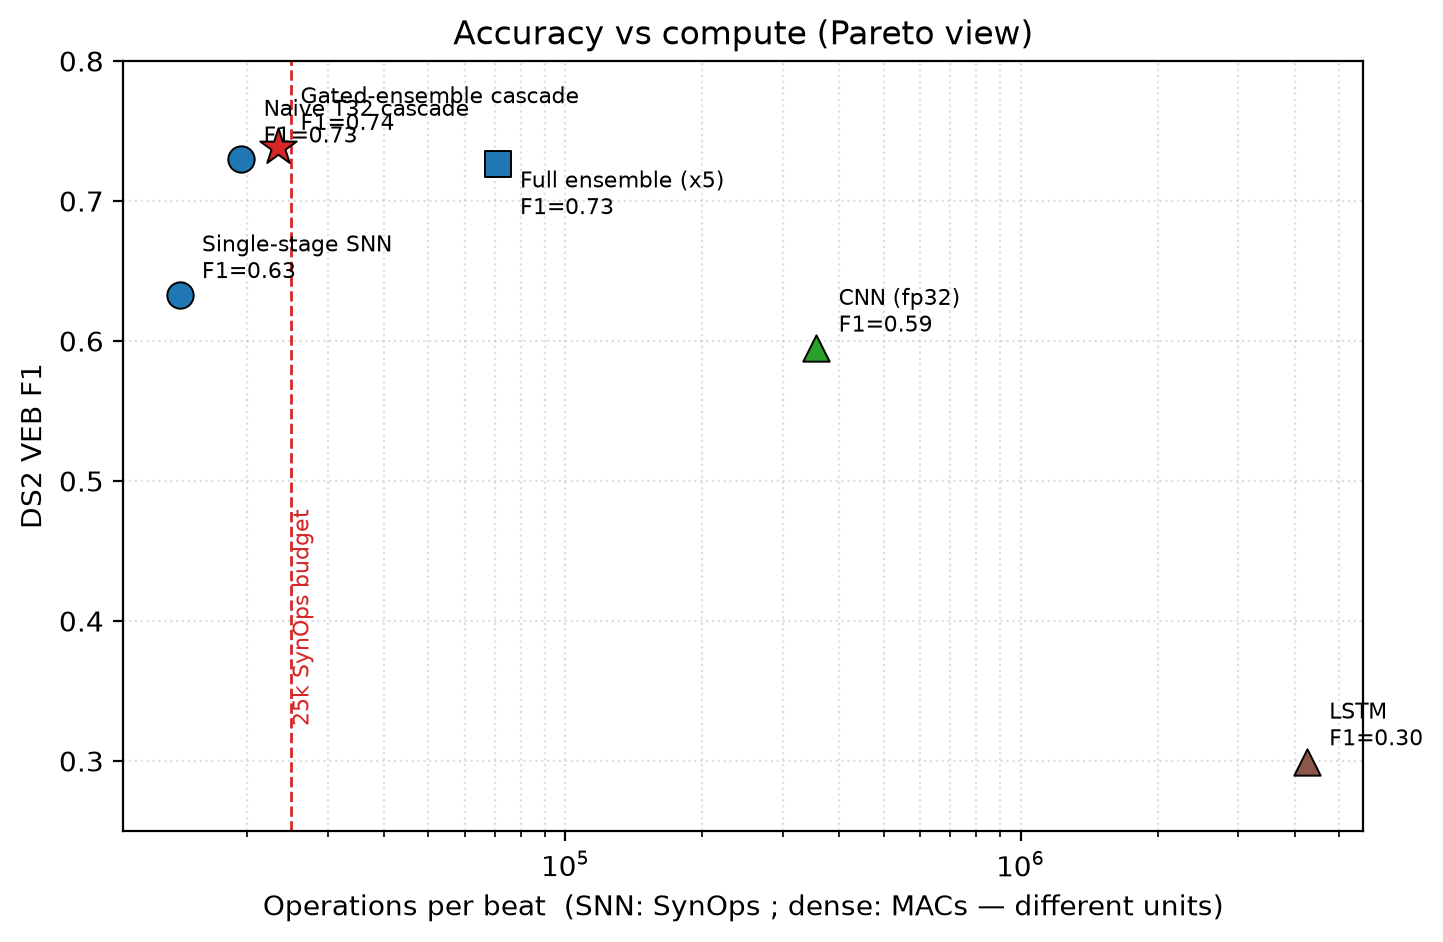
\includegraphics[keepaspectratio]{figures/fig3_pareto.png}}
\caption{Figure 3}
\end{figure}

\textbf{Figure 3 (accuracy-energy Pareto).} DS2 VEB F1 versus operations
per beat, log scale. SNN points are SynOps; CNN and LSTM are MACs, a
different operation unit, and are marked as such. The 25k-SynOps budget
is drawn as a reference line for the SNN points. \emph{Message: the
gated ensemble occupies the within-budget corner; the full ensemble is
more accurate but over budget; the dense baselines sit orders of
magnitude higher in operation count.}

\begin{figure}
\centering
\pandocbounded{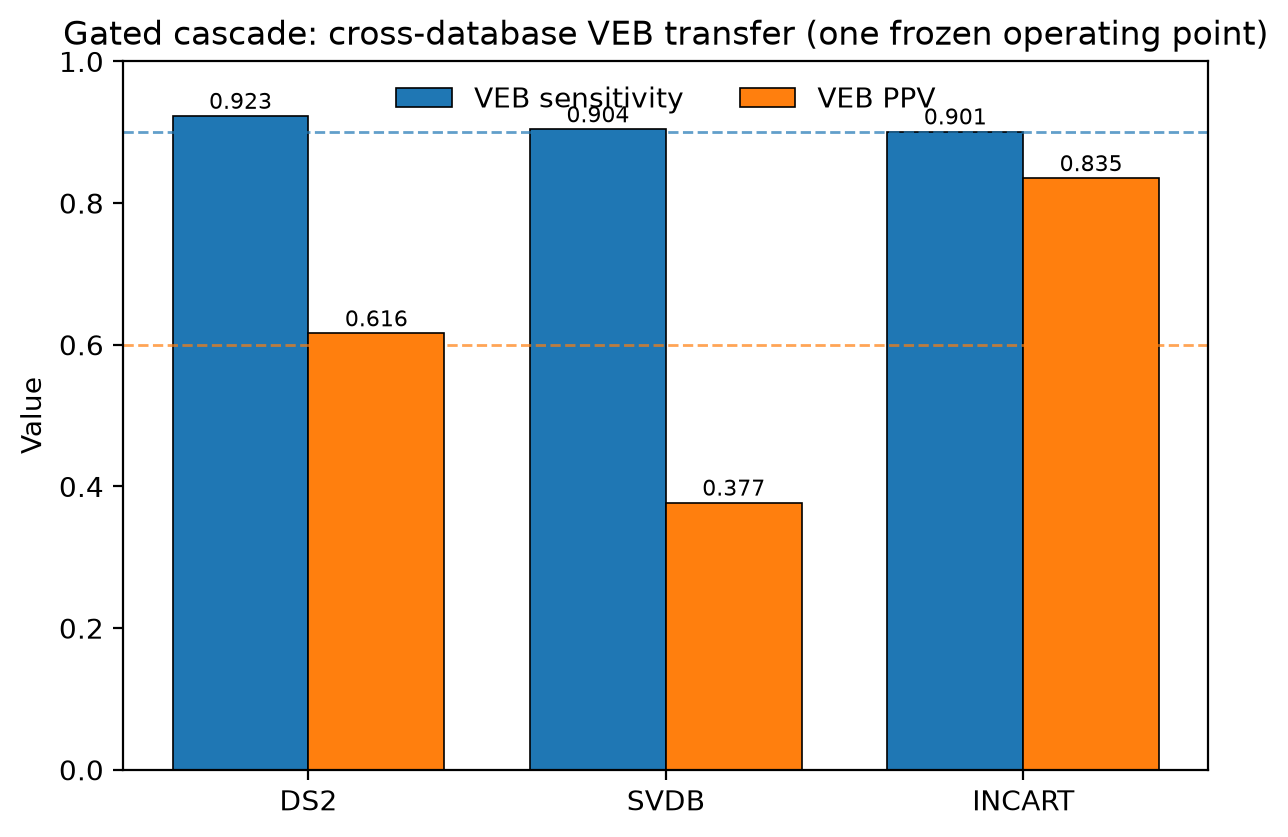
\includegraphics[keepaspectratio]{figures/fig4_crossdb.png}}
\caption{Figure 4}
\end{figure}

\textbf{Figure 4 (cross-database transfer).} VEB sensitivity and PPV for
the frozen gated cascade on DS2, SVDB, and INCART, with the 0.90 and
0.60 target lines. \emph{Message: sensitivity transfers (\textgreater=
0.90 on all three databases under one frozen operating point); PPV
varies with class prevalence.}

\begin{figure}
\centering
\pandocbounded{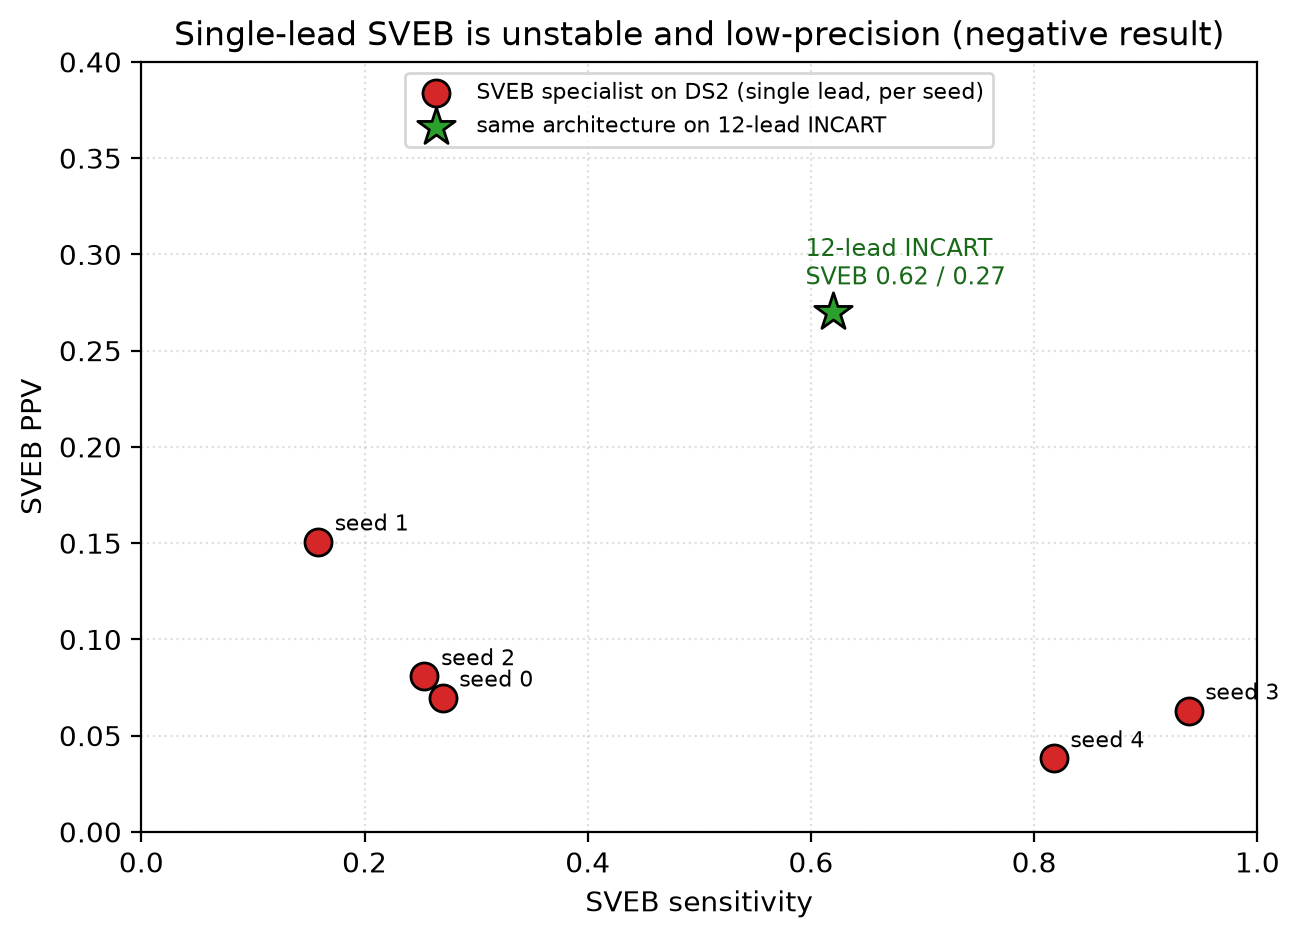
\includegraphics[keepaspectratio]{figures/fig5_sveb.png}}
\caption{Figure 5}
\end{figure}

\textbf{Figure 5 (SVEB negative result).} DS2 SVEB sensitivity versus
PPV per seed for the SVEB specialist (single lead), contrasted with the
same architecture's SVEB detection on 12-lead INCART. \emph{Message:
single-lead SVEB is unstable and low-precision; the same model separates
SVEB far better with more lead information.}

\begin{center}\rule{0.5\linewidth}{0.5pt}\end{center}

\subsection{5. Methods}\label{methods}

\subsubsection{5.1 Spike encoding}\label{spike-encoding}

Each 256-sample beat window is converted to a spike tensor by
count-pooled delta encoding. For each signal order in the set
\texttt{orders} (order 0 is the signal, order 1 its first difference),
threshold crossings of magnitude theta = 0.12 (in normalized signal
units) are accumulated into T time bins, producing two channels (rising
and falling crossings) per order. With \texttt{orders\ =\ {[}0,\ 1{]}}
this yields 2 x \textbar orders\textbar{} = 4 input channels over T
timesteps. Because crossings are pooled by count into bins, the total
number of input spikes over a beat is approximately conserved as T
varies; increasing T redistributes the same spikes into finer bins
rather than creating more of them (Section 8).

\subsubsection{5.2 Network}\label{network}

The classifier is a two-layer LIF network. A linear map \texttt{fc1}
projects the 4 input channels to H = 128 hidden LIF units; a linear map
\texttt{fc2} projects hidden spikes to 5 class logits. The three RR
features are projected once, through a separate dense map, into the
hidden state (they are not re-injected at every timestep). The readout
accumulates the output-layer membrane potential over T timesteps.
Training uses surrogate-gradient backpropagation-through-time (snnTorch
{[}Eshraghian2023{]}, following {[}Neftci2019{]}) with the Adam
optimizer, learning rate 4e-3, 100 epochs, batch size 512, and class
weights scaled as the square root of inverse class frequency to counter
imbalance. Unless stated otherwise the single-stage model uses T = 64.

\subsubsection{5.3 Operating point
selection}\label{operating-point-selection}

The network emits 5 logits; the decision adds a fixed per-class bias
vector \texttt{b\ =\ {[}0,\ b\_S,\ b\_V,\ b\_F,\ b\_Q{]}} and takes the
argmax, with \texttt{b\_F} and \texttt{b\_Q} set to a large negative
constant so that fusion and unknown are never predicted (their support
in DS1 is too small to calibrate). The two free parameters
\texttt{(b\_S,\ b\_V)} are selected by grid search on the validation
holdout only, and then frozen. We define three selection strategies:

\begin{itemize}
\tightlist
\item
  \textbf{sens-first:} maximize validation VEB PPV subject to validation
  VEB sensitivity \textgreater= 0.90;
\item
  \textbf{ppv-first:} maximize validation VEB sensitivity subject to
  validation VEB PPV \textgreater= 0.60;
\item
  \textbf{balanced:} maximize validation VEB F1.
\end{itemize}

When a strategy's constraint is infeasible on validation for a given
seed, we report that seed as infeasible rather than substituting a
degenerate maximum- sensitivity point. The single-stage NeuroBeat-VEB
uses sens-first, because missing ventricular beats is the more costly
error; we also report the full frontier so the tradeoff is explicit.

\subsubsection{5.4 Energy proxy: SynOps per
beat}\label{energy-proxy-synops-per-beat}

We report a per-beat synaptic-operation count, defined as the number of
accumulate operations triggered by spikes across the forward pass:

\texttt{SynOps\ =\ (sum\ over\ T\ of\ input\_spikes)\ *\ H\ +\ (sum\ over\ T\ of\ hidden\_spikes)\ *\ C\ +\ n\_RR\ *\ H},

where H = 128, C = 5, n\_RR = 3, and \texttt{input\_spikes} /
\texttt{hidden\_spikes} are the per-timestep active-unit counts. The
first term (input to hidden) dominates and is encoding-dependent, which
is why sparse, low-order input matters more than T. This proxy counts
the accumulate operations a neuromorphic core performs; it excludes
membrane-state updates, on-chip memory movement, the encoding and sensor
front end, and any host overhead. It is therefore a compute proxy and
not a measured energy figure (Sections 8 and 9). The budget throughout
is 25,000 SynOps/beat.

\subsubsection{5.5 Two-stage gated-ensemble
cascade}\label{two-stage-gated-ensemble-cascade}

A single model cannot reach both target thresholds at one operating
point (Section 7.1). We therefore route inference through two stages:

\begin{itemize}
\tightlist
\item
  \textbf{Screener (every beat).} A deliberately sparse LIF network (T =
  32, H = 64, encoding threshold 0.18, \texttt{orders\ =\ {[}0,\ 1{]}}),
  with its operating point fit on validation for high VEB recall. Its
  sparsity, not its shorter T, is what makes it cheap (Section 8):
  higher threshold and fewer hidden units reduce spike counts, whereas
  reducing T alone would not (Section 5.1).
\item
  \textbf{Confirmer (flagged beats only).} A three-seed ensemble of the
  T = 64 models already trained for the single-stage study, combined by
  logit averaging. It runs only on beats the screener flags. A beat is
  declared VEB if and only if both the screener and the ensemble
  confirmer fire.
\end{itemize}

Both operating points are fit on validation only (screener recall target
0.97; confirmer maximizes cascade VEB PPV subject to cascade VEB
sensitivity \textgreater= 0.90 on validation), then frozen. Average
energy is

\texttt{SynOps(screener)\ +\ flag\_rate\ *\ K\ *\ SynOps(one\ confirmer\ member\ on\ flagged\ beats)},

with K = 3. Because the flag rate is small, the heavier confirmer
contributes little on average. The confirmer members' SynOps are
measured on the flagged (ectopic-enriched) beats, which are more active
and therefore more expensive per beat than an average DS2 beat; we use
that higher figure rather than the DS2-wide average, so the reported
energy is not optimistic.

\subsubsection{5.6 Seeds and model
selection}\label{seeds-and-model-selection}

Each configuration is trained with 5 seeds. For the single-stage frozen
artifact, the seed is chosen by validation VEB F1 among seeds that
satisfy the sens-first validation constraint, never by any DS2 or
external number. For the cascade, the confirmer uses seeds 0 to 2; we
report robustness to this choice in Section 7.3.

\begin{center}\rule{0.5\linewidth}{0.5pt}\end{center}

\subsection{6. Evaluation protocol (no-leakage
statement)}\label{evaluation-protocol-no-leakage-statement}

To make the leakage-control claim unambiguous:

\begin{enumerate}
\def\labelenumi{\arabic{enumi}.}
\tightlist
\item
  DS2 is never used for model selection, hyperparameter selection,
  threshold selection, seed selection, or early stopping. It is
  evaluated once, with a frozen model and a frozen operating point.
\item
  All operating points (single-stage and both cascade stages) are
  selected only on the DS1 validation holdout (records 201, 207, 223),
  which is patient-disjoint from DS1 training.
\item
  SVDB and INCART are test-only. No external beat enters training or
  operating- point selection for the VEB models. Every cross-database
  number uses the same frozen operating point selected on DS1
  validation.
\item
  All reported final numbers were produced by evaluating locked
  artifacts; no number was revised after seeing test performance.
\end{enumerate}

The one deliberate exception is the SVEB specialist (Section 7.6), which
by design adds SVDB and INCART beats to training as an augmentation
study; its DS2 test set remains untouched, and we flag its non-standard
training explicitly.

\begin{center}\rule{0.5\linewidth}{0.5pt}\end{center}

\subsection{7. Results}\label{results}

All results use 5 training seeds. We report seed mean with {[}min,
max{]} where a distribution exists, and 95\% bootstrap confidence
intervals (2,000 resamples over DS2 beats) for the headline cascade. DS2
contains 3,220 VEB beats out of 49,693 (Table 1), so a one-point change
in sensitivity corresponds to about 32 beats.

\subsubsection{7.1 Single-stage VEB
detection}\label{single-stage-veb-detection}

DS2 VEB detection under each validation-fit strategy (5 seeds), with
SynOps/beat:

\begin{longtable}[]{@{}
  >{\raggedright\arraybackslash}p{(\linewidth - 8\tabcolsep) * \real{0.2000}}
  >{\raggedright\arraybackslash}p{(\linewidth - 8\tabcolsep) * \real{0.2000}}
  >{\raggedright\arraybackslash}p{(\linewidth - 8\tabcolsep) * \real{0.2000}}
  >{\raggedright\arraybackslash}p{(\linewidth - 8\tabcolsep) * \real{0.2000}}
  >{\raggedright\arraybackslash}p{(\linewidth - 8\tabcolsep) * \real{0.2000}}@{}}
\toprule\noalign{}
\begin{minipage}[b]{\linewidth}\raggedright
Operating point
\end{minipage} & \begin{minipage}[b]{\linewidth}\raggedright
VEB sensitivity
\end{minipage} & \begin{minipage}[b]{\linewidth}\raggedright
VEB PPV
\end{minipage} & \begin{minipage}[b]{\linewidth}\raggedright
F1
\end{minipage} & \begin{minipage}[b]{\linewidth}\raggedright
SynOps/beat
\end{minipage} \\
\midrule\noalign{}
\endhead
\bottomrule\noalign{}
\endlastfoot
sens-first & 0.905 {[}0.878, 0.928{]} & 0.539 {[}0.490, 0.627{]} & 0.68
& \textasciitilde14,300 \\
balanced & 0.857 {[}0.790, 0.912{]} & 0.679 {[}0.517, 0.780{]} & 0.76 &
\textasciitilde14,300 \\
ppv-first & 0.845 {[}0.771, 0.888{]} & 0.700 {[}0.583, 0.791{]} & 0.77 &
\textasciitilde14,300 \\
\end{longtable}

A single operating point buys sensitivity or precision, not both: at
sensitivity near 0.90 the PPV is about 0.54, and reaching PPV near 0.68
costs roughly 4 to 7 points of sensitivity. All single-stage
configurations sit under the SynOps budget. Note that the balanced point
has a higher F1 (0.76) than the cascade below (0.74): the cascade is not
F1-optimal, it is selected to satisfy both clinical thresholds
(sensitivity \textgreater= 0.90 and PPV \textgreater= 0.60) jointly,
which the balanced point does not (its sensitivity is 0.857).

\textbf{Frontier (Figure 2).} Sweeping the VEB decision threshold on DS2
(an oracle sweep, shown only to characterize what is achievable, not as
an operating point), the DS2 VEB PPV attainable at each sensitivity
level spans, across the 5 seeds:

\begin{longtable}[]{@{}
  >{\raggedright\arraybackslash}p{(\linewidth - 8\tabcolsep) * \real{0.2000}}
  >{\raggedright\arraybackslash}p{(\linewidth - 8\tabcolsep) * \real{0.2000}}
  >{\raggedright\arraybackslash}p{(\linewidth - 8\tabcolsep) * \real{0.2000}}
  >{\raggedright\arraybackslash}p{(\linewidth - 8\tabcolsep) * \real{0.2000}}
  >{\raggedright\arraybackslash}p{(\linewidth - 8\tabcolsep) * \real{0.2000}}@{}}
\toprule\noalign{}
\begin{minipage}[b]{\linewidth}\raggedright
Sensitivity \textgreater=
\end{minipage} & \begin{minipage}[b]{\linewidth}\raggedright
0.80
\end{minipage} & \begin{minipage}[b]{\linewidth}\raggedright
0.85
\end{minipage} & \begin{minipage}[b]{\linewidth}\raggedright
0.90
\end{minipage} & \begin{minipage}[b]{\linewidth}\raggedright
0.92
\end{minipage} \\
\midrule\noalign{}
\endhead
\bottomrule\noalign{}
\endlastfoot
VEB PPV (range) & 0.57 to 0.78 & 0.57 to 0.69 & 0.56 to 0.65 & 0.48 to
0.57 \\
\end{longtable}

Two of the five seeds cannot exceed 0.90 sensitivity on DS2 even at the
oracle threshold, and no seed offers a single point at both sensitivity
\textgreater= 0.90 and PPV \textgreater= 0.60 with margin. This
motivates the cascade.

\subsubsection{7.2 Cross-database generalization
(single-stage)}\label{cross-database-generalization-single-stage}

The frozen single-stage model (sens-first, fit on DS1 validation)
applied unchanged:

\begin{longtable}[]{@{}lrrll@{}}
\toprule\noalign{}
Database & Beats & VEB beats & VEB sensitivity & VEB PPV \\
\midrule\noalign{}
\endhead
\bottomrule\noalign{}
\endlastfoot
MIT-BIH DS2 & 49,693 & 3,220 & 0.894 & 0.490 \\
MIT-BIH SVDB & 184,520 & 9,941 & 0.892 & 0.361 \\
INCART & 175,811 & 20,006 & 0.880 & 0.736 \\
\end{longtable}

VEB sensitivity holds in a narrow band (0.88 to 0.89) across three
databases with different patients, leads, and original sampling rates,
under one frozen operating point. PPV varies with class prevalence: it
is lower on the supraventricular-dense SVDB (more non-VEB beats
resembling VEB) and higher on the VEB-dense INCART. This is the expected
behaviour of a fixed threshold under prevalence shift and is why we
report sensitivity and PPV separately rather than a single accuracy
figure.

\subsubsection{7.3 Two-stage gated-ensemble
cascade}\label{two-stage-gated-ensemble-cascade-1}

The frozen cascade (screener recall target 0.97; confirmer fit for
cascade PPV subject to cascade sensitivity \textgreater= 0.90; both on
validation only):

\begin{longtable}[]{@{}lrrlll@{}}
\toprule\noalign{}
Database & Beats & VEB beats & VEB sensitivity & VEB PPV & Flag rate \\
\midrule\noalign{}
\endhead
\bottomrule\noalign{}
\endlastfoot
MIT-BIH DS2 & 49,693 & 3,220 & 0.923 & 0.616 & 0.271 \\
MIT-BIH SVDB & 184,520 & 9,941 & 0.904 & 0.377 & 0.345 \\
INCART & 175,811 & 20,006 & 0.901 & 0.835 & 0.241 \\
\end{longtable}

We report two bootstrap intervals for the DS2 point estimates. A
beat-level bootstrap (resampling beats independently, 2,000 resamples)
gives sensitivity {[}0.914, 0.932{]} and PPV {[}0.602, 0.630{]}. A
patient-level bootstrap (resampling the 22 DS2 records with replacement,
which respects within-record correlation) gives much wider intervals:
sensitivity {[}0.850, 0.976{]} and PPV {[}0.355, 0.814{]}. The gap
between the two is large because VEB beats are concentrated in a
minority of records, so a few patients dominate the estimate. The
patient-level interval is the honest one to quote: the point estimates
meet the targets on DS2's specific patient composition, but per-patient
behaviour varies substantially, and a wider prospective evaluation would
be needed to tighten this. Average energy on DS2 is
\texttt{5,987\ +\ 0.271\ *\ 3\ *\ 21,433\ =\ 23,385} SynOps/beat, within
the 25,000 budget. Robustness to the confirmer composition: ensembles of
K in \{2, 3, 5\} members and different 3-member subsets all give DS2
sensitivity \textgreater= 0.90 at PPV between 0.59 and 0.64.

\subsubsection{7.4 Accuracy-energy Pareto (Figure
3)}\label{accuracy-energy-pareto-figure-3}

\begin{longtable}[]{@{}lll@{}}
\toprule\noalign{}
Model & DS2 sens / PPV & Compute/beat \\
\midrule\noalign{}
\endhead
\bottomrule\noalign{}
\endlastfoot
Single-stage (sens-first) & 0.894 / 0.490 & 14,200 SynOps \\
Naive T32 cascade & 0.883 / 0.622 & 19,400 SynOps \\
Full 5-seed ensemble (every beat) & 0.932 / 0.595 &
\textasciitilde71,000 SynOps \\
Gated-ensemble cascade & 0.923 / 0.616 & 23,385 SynOps \\
\end{longtable}

The full ensemble reaches the target corner but costs about five forward
passes and exceeds the budget. The gated cascade recovers most of that
accuracy within budget by running the ensemble only on flagged beats.
The naive T32 cascade is a cautionary point: it costs more than the
single-stage model, because a shorter network is not a cheaper one under
count-pooled encoding (Section 8).

\subsubsection{7.5 Non-spiking baselines on the same
split}\label{non-spiking-baselines-on-the-same-split}

We train 1-D CNN and LSTM baselines under the identical protocol: same
DS1 train, same beat-plus-RR inputs, same validation-locked sens-first
operating point, same frozen DS2 test, 5 seeds.

\begin{longtable}[]{@{}lllll@{}}
\toprule\noalign{}
Model & DS2 sens & DS2 PPV & Operations/beat & Params \\
\midrule\noalign{}
\endhead
\bottomrule\noalign{}
\endlastfoot
CNN (1-D, beat+RR) & 0.945 {[}0.926, 0.959{]} & 0.434 & 356k MACs &
2.9k \\
LSTM (beat+RR) & 0.940 {[}0.911, 0.974{]} & 0.178 & 4.26M MACs &
17.5k \\
SNN single-stage & 0.894 & 0.490 & 14.2k SynOps & 18k \\
SNN gated-ensemble & 0.923 & 0.616 & 23.4k SynOps & n/a \\
\end{longtable}

Two observations. First, the dense baselines show the same
sensitivity/precision tradeoff: under the sens-first operating point
they reach high sensitivity (about 0.94) but low PPV (0.43 for the CNN,
0.18 for the LSTM), so the tradeoff is a property of single-lead VEB
detection rather than of spiking networks. Second, on operation count
the SNN is far lower: 14k to 23k SynOps versus 356k (CNN) and 4.26M
(LSTM) MACs. We state this carefully. A SynOp (a spike-triggered
accumulate) and a MAC (a multiply-accumulate) are not the same unit, and
this comparison is an operation-count advantage under a proxy model, not
a measured energy ratio. The comparison would be strengthened by
quantized CNN and temporal-convolutional baselines and by measured
microcontroller energy (Section 9). Within these caveats, the gated
cascade also attains the highest PPV of any model at comparable
sensitivity.

Post-training int8 weight quantization of the CNN (per-tensor symmetric,
weights only, activations left in float, 3 seeds) preserves DS2 VEB
detection: fp32 0.951 / 0.417 versus int8 0.951 / 0.444 (sensitivity /
PPV), with weight memory reduced from 11.6 kB to 3.1 kB. This is the
fair embedded operating point for the dense baseline: the MAC count is
unchanged (356k/beat), but an int8 MAC is materially cheaper and smaller
than an fp32 MAC on typical microcontrollers. Quantization therefore
closes part of the compute gap in energy-per-operation terms without
changing the operation count, and a full int8 pipeline (quantized
activations, with calibration) plus measured board energy is the
comparison we recommend for a camera-ready version (Section 9).

\subsubsection{7.6 Supraventricular beats: a single-lead negative
result}\label{supraventricular-beats-a-single-lead-negative-result}

Supraventricular ectopic beats often differ from normal beats mainly in
timing and subtle morphology, and DS1 contains few of them (Table 1). As
an incidental output of the VEB model, DS2 SVEB sensitivity is about
0.13; adding supraventricular-rich SVDB to training raises it to about
0.24, and a higher-time-resolution variant to about 0.27, all still low.

We then trained a dedicated SVEB specialist (higher time resolution,
SVDB and INCART added to training, an SVEB-first operating point, 5
seeds). It does not yield a usable detector:

\begin{longtable}[]{@{}
  >{\raggedright\arraybackslash}p{(\linewidth - 6\tabcolsep) * \real{0.2500}}
  >{\raggedright\arraybackslash}p{(\linewidth - 6\tabcolsep) * \real{0.2500}}
  >{\raggedright\arraybackslash}p{(\linewidth - 6\tabcolsep) * \real{0.2500}}
  >{\raggedright\arraybackslash}p{(\linewidth - 6\tabcolsep) * \real{0.2500}}@{}}
\toprule\noalign{}
\begin{minipage}[b]{\linewidth}\raggedright
Seed regime
\end{minipage} & \begin{minipage}[b]{\linewidth}\raggedright
DS2 SVEB sens
\end{minipage} & \begin{minipage}[b]{\linewidth}\raggedright
DS2 SVEB PPV
\end{minipage} & \begin{minipage}[b]{\linewidth}\raggedright
DS2 VEB sens
\end{minipage} \\
\midrule\noalign{}
\endhead
\bottomrule\noalign{}
\endlastfoot
calibrated (seeds 0 to 2) & 0.16 to 0.27 & 0.07 to 0.15 & degraded \\
degenerate (seeds 3 to 4) & 0.82 to 0.94 & 0.04 to 0.06 & 0.18 to
0.24 \\
\end{longtable}

The high-sensitivity seeds reach it only by flagging almost all beats as
SVEB (PPV at or below 0.06), which collapses the ventricular class. DS2
SVEB PPV never exceeds about 0.15 at any operating point, and the
outcome is unstable across seeds. The same architecture reaches SVEB
sensitivity 0.62 on 12-lead INCART, which indicates that the limiting
factor is available lead information and data rather than model
capacity. We therefore treat single-lead SVEB as an open problem and,
importantly, do not allow it to reshape the VEB operating point.
Multi-lead input (MIT-BIH provides a second lead; supraventricular beats
separate better on some leads) and richer SVEB training data are the
natural next steps (Section 9).

\begin{center}\rule{0.5\linewidth}{0.5pt}\end{center}

\subsection{8. Discussion}\label{discussion}

\textbf{(a) Honest evaluation lowers headline numbers but increases
trust.} Freezing the operating point on validation rather than test, and
reporting inter-patient rather than intra-patient results, lowers our
headline metrics relative to test-tuned or intra-patient reports. The
compensating evidence is transfer: the same frozen operating point holds
VEB sensitivity at or above 0.90 across three databases, which a
test-tuned threshold cannot promise. We regard the frozen cross-database
result as the most decision-relevant number in the paper.

\textbf{(b) Energy-accounted models need explicit budgets.} Reporting
SynOps for every configuration, and enforcing a fixed budget, changes
which design choices look attractive. It is what exposes the naive
cascade as a false economy and the full ensemble as over budget, and it
is what makes the sparse-screener design necessary rather than
incidental.

\textbf{(c) Time resolution is not the same as energy cost under
count-pooled encoding.} Because count-pooling approximately conserves
total input spikes across T, the dominant SynOps term is roughly
independent of T. Two consequences follow: raising T sharpens
discrimination at almost no energy cost, and a shorter network is not a
cheaper one. A screener must be made cheap by reducing channels, hidden
units, or spike rate (via a higher threshold), which is exactly how our
screener is built.

\textbf{(d) The cascade addresses a calibration-variance limit at low
average cost.} The DS2 oracle frontier shows that sensitivity
\textgreater= 0.90 at PPV \textgreater= 0.60 is attainable, yet single
models calibrated on a small validation holdout land there only
occasionally and vary across seeds. A small ensemble both reduces model
variance and calibrates more stably, reaching 0.918 / 0.634 on DS2 for
three members; gating it behind a sparse screener delivers that accuracy
within budget.

\textbf{(e) VEB is promising; single-lead SVEB is not solved.} The VEB
result is usable under a strict protocol and an energy budget. The SVEB
result is a clean negative under the same protocol, and we present it as
such.

\textbf{Alternative explanations we cannot fully exclude.} The
cross-database PPV differences could reflect annotation-convention
differences between databases rather than only prevalence. The
single-model seed variance could partly reflect optimization noise
rather than only calibration; the ensemble would help in either case. We
report both beat-level and patient-level bootstrap intervals (Section
7.3); the patient-level interval is much wider because a few records
dominate the DS2 VEB count, and it is the interval we treat as the
honest uncertainty.

\begin{center}\rule{0.5\linewidth}{0.5pt}\end{center}

\subsection{9. Limitations}\label{limitations}

\begin{itemize}
\tightlist
\item
  \textbf{SynOps is a compute proxy, not measured energy.} Actual joules
  depend on the target chip, on-chip and off-chip memory movement, the
  compiler and runtime, the sensor and encoding front end, and the
  specific implementation. We report no measured hardware energy.
\item
  \textbf{Retrospective public data only.} All data are curated public
  research databases with expert beat annotations. Performance on raw,
  artefact-laden device recordings is untested.
\item
  \textbf{Small validation holdout.} Three DS1 records make single-model
  operating points noisy; the ensemble mitigates but does not remove
  this. A larger or cross-validated holdout is likely to tighten
  calibration.
\item
  \textbf{Detection is conditional on R-peak annotations.} We use
  provided annotations and do not include a beat detector; end-to-end
  performance would also depend on detector errors.
\item
  \textbf{Prevalence-dependent PPV.} Cross-database PPV is sensitive to
  class composition, so PPV numbers should be read together with the
  beat counts.
\item
  \textbf{Single lead.} Results use one lead; SVEB in particular appears
  to need more lead information.
\item
  \textbf{Large between-patient variance.} With only 22 DS2 patients, a
  patient-level bootstrap gives wide intervals (VEB sensitivity 0.85 to
  0.98, PPV 0.36 to 0.81). The point estimates hold for DS2's
  composition, but per-patient behaviour varies substantially, so a
  larger prospective cohort is needed to tighten them.
\item
  \textbf{No prospective or clinical-workflow validation, and no
  subgroup or demographic fairness analysis.} Nothing here has been
  validated in a deployment or against regulatory-grade endpoints.
\end{itemize}

\begin{center}\rule{0.5\linewidth}{0.5pt}\end{center}

\subsection{10. Clinical and commercial
relevance}\label{clinical-and-commercial-relevance}

The most credible near-term role for this work is as a low-power VEB
screening component inside a larger pipeline: wearable or patch ECG,
Holter-style ambulatory monitoring, remote patient monitoring, or a
neuromorphic edge inference block that flags ventricular ectopy for
downstream review. In such a role, high sensitivity at a controlled
compute budget, with predictable cross-database behaviour, is the
relevant property, and PPV in the 0.6 range is acceptable for a
screening stage that feeds human or higher-tier automated review.

We make no claim of diagnostic readiness. A path to product would
require, at minimum, measured energy on the intended microcontroller or
neuromorphic hardware, prospective validation on device-quality
recordings, integration into a clinical workflow with defined alarm
handling, quality-system and software-as-a-medical- device processes,
and a regulatory strategy. The present contribution is a methodological
and feasibility result, not a cleared device.

\begin{center}\rule{0.5\linewidth}{0.5pt}\end{center}

\subsection{11. Conclusion}\label{conclusion}

NeuroBeat shows that a compact, conventional spiking network, evaluated
under a conservative validation-locked inter-patient protocol and held
to an explicit per-beat SynOps budget, can reach useful
ventricular-ectopic-beat sensitivity and precision (0.923 sensitivity at
0.616 PPV on MIT-BIH DS2, within 23,385 SynOps/beat) using a
gated-ensemble cascade, while transferring at or above 0.90 sensitivity
to two unseen databases under one frozen operating point. The main
contribution is not a new architecture but an honest, energy-accounted
evaluation pattern for low-power ECG detection, together with a clearly
reported negative result for single-lead supraventricular detection. We
hope the protocol, the SynOps budgeting, and the released artifacts are
reusable by others reporting SNN-ECG results.

\begin{center}\rule{0.5\linewidth}{0.5pt}\end{center}

\subsection{12. Reproducibility}\label{reproducibility}

\begin{itemize}
\tightlist
\item
  Repository: github.com/Talch87/neuro-beat (AGPL-3.0 / commercial dual
  license)
\item
  Live results page: talch87.github.io/neuro-beat
\item
  Frozen artifacts: \texttt{models/neurobeat-veb-v1/} (single-stage
  weights and operating point, sparse screener, three confirmer members,
  gated-cascade configuration, model card)
\item
  Protocol harnesses: \texttt{experiments/freeze\_veb\_v1.py}
  (single-stage; \texttt{-\/-refit-only} re-tunes the operating point
  from cache), \texttt{experiments/gated\_ensemble\_veb.py} (cascade),
  \texttt{experiments/baselines\_veb.py} (CNN/LSTM)
\item
  All experiments use 5 seeds with the operating point fit on DS1
  validation only.
\end{itemize}

\begin{center}\rule{0.5\linewidth}{0.5pt}\end{center}

\subsection{References}\label{references}

\emph{Compiled and cross-checked against source pages (arXiv, PubMed)
and literature search, July 2026. The Neurocomputing entry's author list
is from a secondary search and should be confirmed against the publisher
page.}

\begin{itemize}
\tightlist
\item
  \textbf{{[}AAMI-EC57{]}} ANSI/AAMI EC57. \emph{Testing and Reporting
  Performance Results of Cardiac Rhythm and ST-Segment Measurement
  Algorithms.} Association for the Advancement of Medical
  Instrumentation.
\item
  \textbf{{[}deChazal2004{]}} P. de Chazal, M. O'Dwyer, R. B. Reilly.
  ``Automatic classification of heartbeats using ECG morphology and
  heartbeat interval features.'' \emph{IEEE Trans. Biomed. Eng.},
  51(7):1196 to 1206, 2004. doi:10.1109/TBME.2004.827359.
\item
  \textbf{{[}Silva2025{]}} G. Silva, P. Silva, G. Moreira, V. Freitas,
  J. Gertrudes, E. Luz. ``A Systematic Review of ECG Arrhythmia
  Classification: Adherence to Standards, Fair Evaluation, and Embedded
  Feasibility.'' arXiv:2503.07276, 2025.
\item
  \textbf{{[}Moody2001{]}} G. B. Moody, R. G. Mark. ``The impact of the
  MIT-BIH Arrhythmia Database.'' \emph{IEEE Eng. Med. Biol. Mag.},
  20(3):45 to 50, 2001.
\item
  \textbf{{[}Goldberger2000{]}} A. L. Goldberger et al.~``PhysioBank,
  PhysioToolkit, and PhysioNet.'' \emph{Circulation}, 101(23):e215 to
  e220, 2000.
\item
  \textbf{{[}Neftci2019{]}} E. O. Neftci, H. Mostafa, F. Zenke.
  ``Surrogate Gradient Learning in Spiking Neural Networks.'' \emph{IEEE
  Signal Process. Mag.}, 36(6):51 to 63, 2019.
\item
  \textbf{{[}Eshraghian2023{]}} J. K. Eshraghian et al.~``Training
  Spiking Neural Networks Using Lessons From Deep Learning.''
  \emph{Proc. IEEE}, 111(9):1016 to 1054, 2023.
\item
  \textbf{{[}Davies2018{]}} M. Davies et al.~``Loihi: A Neuromorphic
  Manycore Processor with On-Chip Learning.'' \emph{IEEE Micro},
  38(1):82 to 99, 2018.
\item
  \textbf{{[}SNN-ECG-BSPC2021{]}} Z. Yan, J. Zhou, W.-F. Wong. ``Energy
  efficient ECG classification with spiking neural network.''
  \emph{Biomed. Signal Process. Control}, 63:102170, 2021.
  doi:10.1016/j.bspc.2020.102170.
\item
  \textbf{{[}Chu2022{]}} H. Chu, Y. Yan, L. Gan, H. Jia, L. Qian, Y.
  Huan, L. Zheng, Z. Zou. ``A Neuromorphic Processing System With
  Spike-Driven SNN Processor for Wearable ECG Classification.''
  \emph{IEEE Trans. Biomed. Circuits Syst.}, 2022. (PubMed 35802543.)
\item
  \textbf{{[}SparrowSNN2024{]}} Z. Yan, Z. Bai, T. Mitra, W.-F. Wong.
  ``SparrowSNN: A Hardware/Software Co-design for Energy Efficient ECG
  Classification.'' arXiv:2406.06543, 2024.
\item
  \textbf{{[}AxonalDelays2025{]}} J. Galvis-Chacon, O. Ramos-Soto, D.
  Oliva, A. Patino-Saucedo. ``Robust ECG signal classification using
  spiking neural networks with axonal delays.'' \emph{Neurocomputing},
  2025. (ScienceDirect S0925231225029315; author list from secondary
  search, to confirm.)
\end{itemize}

\end{document}
